\documentclass[10pt, conference, compsocconf]{llncs}
% Add the compsocconf option for Computer Society conferences.
%
% If IEEEtran.cls has not been installed into the LaTeX system files,
% manually specify the path to it like:
% \documentclass[conference]{../sty/IEEEtran}
\newcommand{\highlight}[1]{\colorbox{yellow}{#1}}


% Some very useful LaTeX packages include:

% *** MISC UTILITY PACKAGES ***
%
\usepackage{ifpdf}


% *** CITATION PACKAGES ***
%
%\usepackage{cite}


% *** MATH PACKAGES ***
%
\usepackage[cmex10]{amsmath}
\usepackage{amssymb}

% *** SPECIALIZED LIST PACKAGES ***
%
\usepackage{algorithmic}

% *** ALIGNMENT PACKAGES ***
%
\usepackage{array}

% *** SUBFIGURE PACKAGES ***
%
\usepackage[tight,footnotesize]{subfigure}

% *** FLOAT PACKAGES ***
%
\usepackage{fixltx2e}
\usepackage{stfloats}

% *** GRAPHICS PACKAGES ***
%
\usepackage{graphicx}

% *** BIBLIOGRAPHY PACKAGES ***
%
\usepackage{natbib}

% *** LANGUAGE PACKAGES ***
%
\usepackage[utf8]{inputenc} 
\usepackage[T1]{fontenc}      
\usepackage[francais]{babel}

% *** LAYOUT PACKAGES ***
%
\usepackage[top=4cm, bottom=4cm, left=4cm, right=4cm]{geometry}


\begin{document}
%
% paper title
% can use linebreaks \\ within to get better formatting as desired
\title{Snakebites Monitoring System}





% author names and affiliations
% use a multiple column layout for up to two different
% affiliations
% 
\author{Djavan Sergent \\
Master en Sciences Informatiques \\
 djavan.sergent@etu.unige.ch}

\institute{Université de Genève}



% make the title area
\maketitle


\textbf{Mots clés}
snakebite ; monitoring \\
\\
Une application qui permet d'identifier et de retracer la migration des espèces de serpents impliquées dans les attaques pour une meilleure prise en charge des victimes. \\
\\
Les serpents sont responsables chaque année de milliers de morts à travers le monde. Celles-ci sont estimées entre 20'000 et 90'000 \cite{kasturiratne_global_2008}. Un tel écart s'explique par l'absence d'obligation de rapporter le nombre de victimes dans de nombreux pays, ce qui empêche toute étude à un niveau international. De plus, la mort est parfois due à l'impossibilité d'administrer le bon antidote. En permettant d'identifier l'espèce et de signaler les zones dangereuses avec un smartphone on pourrait mieux recenser ainsi que diminuer la gravité des attaques. \\
\begin{figure}
	\begin{center}
		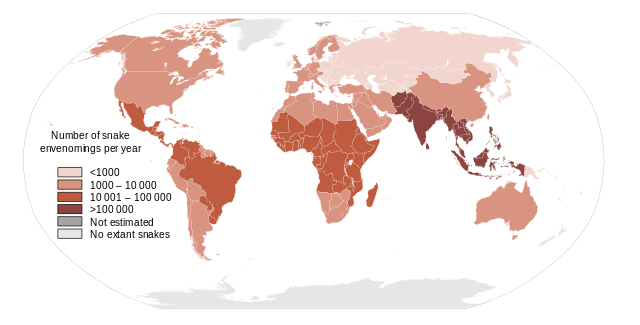
\includegraphics[width=200pt]{snake.png}
	\end{center}
	\caption{Répartition des morsures (source : Wikipedia)}
\end{figure}
\\
Aujourd'hui, la majorité des cas de morsures ne sont pas traités correctement en Afrique sub-saharienne car les populations préfèrent se fier aux médecines traditionnelles \cite{noauthor_epidemiology_2017}. Les victimes attendent parfois jusqu'à plusieurs semaines avant de se rendre chez un médecin, ce qui peut mener à de graves lésions permanentes et à des handicaps \cite{chippaux_snake-bites:_2009}. De plus, le manque d'informations concernant les dangers de l'espèce impliquée est un problème lorsqu'il s'agit de déterminer quel est l'antidote approprié \cite{gutierrez_trends_2007}. Une prise en charge rapide est essentielle pour diminuer les risques à long terme. Enfin, l'accès aux antidotes est difficile et souvent onéreux pour les populations les plus exposées. \\
\\
Il est donc important d'aider les victimes à déterminer au plus vite la gravité de la morsure pour que celles-ci aient toutes les informations nécessaires à la prise de décision de se rendre ou non chez un médecin. Il est également très important d'informer la population des répartitions des zones à risques pour qu'elle puisse connaître et emprunter les itinéraires les moins dangereux et d'obtenir une vision globale des cas de morsures. \\
\\
Une approche possible serait de récolter des informations au moment de la morsure au moyen d'une application. Celle-ci conserverait localement les coordonnées GPS ainsi qu'une photo du serpent et/ou de la blessure et comparerait avec sa base de données d'images afin de tenter de déterminer l'espèce qui a attaqué. Avec cette information la victime peut immédiatement déterminer la gravité de la situation. Dans un second temps, lors d'une prise en main médicale, le médecin peut rapidement identifier le bon antidote à administrer. Lorsque l'utilisateur de l'application dispose d'un accès internet, les données sont envoyées sur un serveur afin d'en extraire un certain nombre de d'informations et statistiques comme par exemple la répartition géographique des différentes espèces. \\
\\
Dans notre cas, l'application doit pouvoir fonctionner en autonomie dans les régions qui ne disposent pas d'un accès internet. Elle doit également permettre d'envoyer les données sur le réseau au moyen d'une connexion sans fil. L'application doit également être capable d'analyser les photos et d'en tirer les caractéristiques principales permettant d'identifier l'espèce du reptile. On pourrait utiliser une combinaison d'informations manuelles (taille estimée, couleurs etc.) et d'extraction automatique pour déterminer au mieux quel type de serpent est impliqué. L'application pourrait également par la suite envoyer une notification à un utilisateur s'approchant d'une zone réputée dangereuse.\\
\\
On sait que la très grande majorité des serpents ne sont pas venimeux, et qu'une fraction seulement peut provoquer la mort du patient\cite{simpson_snakes_2007}. Les données relatives aux morsures pourraient permettre d'identifier les zones à risques élevés. Une étude de l'évolution dans le temps de la position des zones à risques et des différents facteurs qui peuvent mener les serprents à migrer serait un outil important pour déterminer les mesures à prendre pour protéger les populations vulnérables. La répartition des antidotes pourrait ainsi être fortement optimisée pour répondre aux besoins concrets des différentes régions. Une meilleure identification des cas de morsures permettrait également d'obtenir des statistiques régionales, nationales et internationales. \\
\\
Pour déterminer l'efficacité d'un tel système, on peut évaluer la qualité de la reconnaissance d'images au travers de sa précision et l'améliorer en utilisant les différentes techniques d'analyse des composantes principales couplées aux informations saisies manuellement. On peut également demander à l'utilisateur si les informations fournies lui ont été utiles ou non. L'analyse approfondie des différentes statistiques permettrait d'accéder à des informations internationales, fiables et standardisées. Il s'agirait alors du premier outil permettant de déterminer statistiquement, en fonction de la région et des symptômes liés à la morsure, l'espèce probablement impliquée. \\
\\
En résumé, cette application se veut être un outil de prise de décision : prise ou non de rendez-vous médical, choix de l'antidote, choix de l'itinéraire, mesures à prendre pour protéger les populations vulnérables, etc. Ces éléments sont essentiels pour réduire la gravité et la fréquence des attaques. A cela s'ajoute la possibilité d'étudier à différents niveaux la répartition des zones dangereuses et d'en tirer les informations nécessaires à une meilleure répartition des stocks, finis, d'antidotes. Un tel système disposerait d'un bon potentiel pour améliorer la santé des personnes à travers le monde de façon globale et plus particulièrement dans les zones agricoles.\\
\\
\textbf{Nombre de mots : 802}
\\ 
\bibliographystyle{plain}
\bibliography{bib} %%% bib.bib is the file containing bibliographic entries
\end{document}